
\de{ĐỀ THI GIỮA HỌC KỲ I NĂM HỌC 2023-2024}{THPT Nguyễn Du}
\begin{center}
	\textbf{PHẦN 1 - TRẮC NGHIỆM}
\end{center}
\Opensolutionfile{ans}[ans/ans]
%===================================
%Câu 1
\begin{ex}%[0D1N2-3]%[Dự án đề kiểm tra Toán 10 GHKI NH23-24- Nguyễn Đức Lợi]%[THPT Nguyễn Du]
	Sử dụng các kí hiệu khoảng, nửa khoảng, đoạn để viết tập hợp $A = \{x \in \mathbb{R} \mid 4 \le x \le 9 \}$.
	\choice
	{$A = [4;9)$}
	{$A = (4;9)$}
	{\True $A = [4;9]$}
	{$A = (4;9]$}
	\loigiai{
		Ta có $A = \{x \in \mathbb{R} \mid 4 \le x \le 9 \} = [4;9]$.
	}
\end{ex}
%===================================
%Câu 2
\begin{ex}%[0H4N1-3]%[Dự án đề kiểm tra Toán 10 GHKI NH23-24- Nguyễn Đức Lợi]%[THPT Nguyễn Du]
	Khẳng định nào sau đây đúng?
	\choice
	{$\tan \alpha = \tan (180^\circ - \alpha)$}
	{$\cos \alpha = \cos (180^\circ - \alpha)$}
	{$\cot \alpha = \cot (180^\circ - \alpha)$}
	{\True $\sin\alpha = \sin (180^\circ - \alpha)$}
	\loigiai{
		Ta có $\sin\alpha = \sin (180^\circ - \alpha)$.
	}
\end{ex}
%===================================
%Câu 3
\begin{ex}%[0H4H2-1]%[Dự án đề kiểm tra Toán 10 GHKI NH23-24- Nguyễn Đức Lợi]%[THPT Nguyễn Du]
	Cho tam giác $ABC$ có $\widehat{BAC} = 30^\circ$ và $BC = 10$. Bán kính đường tròn ngoại tiếp tam giác $ABC$ là
	\choice
	{\True $R = 10$}
	{$R = 5$}
	{$R = 10\sqrt{3}$}
	{$R = \dfrac{10}{\sqrt{3}}$}
	\loigiai{
		Áp dụng định lý sin trong tam giác $ABC$ ta có 
		$$\dfrac{BC}{\sin A} = 2R \Rightarrow R = \dfrac{BC}{2\sin A} = \dfrac{10}{2\sin 30^\circ} = 10.$$
	}
\end{ex}
%===================================
%Câu 4
\begin{ex}%[0D2N1-1]%[Dự án đề kiểm tra Toán 10 GHKI NH23-24- Nguyễn Đức Lợi]%[THPT Nguyễn Du]
	Hệ bất phương trình nào sau đây \textbf{không} là hệ bất phương trình bậc nhất hai ẩn?
	\choice
	{$\heva{& x-2y \le 0 \\ & x + 3y \ge -2}$}
	{$\heva{& x-y > 0 \\ & x - 3y +3 < 0 \\ & x + y -5 > 0}$}
	{\True $\heva{& 3-y < 0 \\ & 2x^2 - 3y + 1> 0}$}
	{$\heva{& 2x-1 \le 0 \\ & 3x + 5 \le 0}$}
	\loigiai{
		Vì trong hệ $\heva{& 3-y < 0 \\ & 2x^2 - 3y + 1> 0}$ có bất phương trình $2x^2 - 3y + 1> 0$ nên hệ đó không là hệ bất phương trình bậc nhất hai ẩn.
	}
\end{ex}

%===================================
%Câu 5
\begin{ex}%[0D2H1-2]%[Dự án đề kiểm tra Toán 10 GHKI NH23-24- Nguyễn Đức Lợi]%[THPT Nguyễn Du]
	Miền nghiệm của bất phương trình $3x + 2(y+3) \ge 4(x+1)-y+3$ chứa điểm nào trong các điểm sau?
	\choice
	{$A(3;1)$}
	{\True $B(2;1)$}
	{$C(3;0)$}
	{$O(3;0)$}
	\loigiai{
		Thay tọa độ các điểm vào bất phương trình đã cho ta thấy điểm $B(2;1)$ thỏa mãn.
	}
\end{ex}

%===================================
%Câu 6
\begin{ex}%[0D1H3-2]%[Dự án đề kiểm tra Toán 10 GHKI NH23-24- Nguyễn Đức Lợi]%[THPT Nguyễn Du]
	Cho hai tập hợp $A = \{x\in \mathbb{N} \mid (x-2)(x^2+3x-4) = 0 \}$ và $B = \{x \in \mathbb{Z} \mid |x-3| \le 1 \}$. Tập $A\setminus B $ có bao nhiêu phần tử?
	\choice
	{$4$}
	{\True $1$}
	{$3$}
	{$2$}
	\loigiai{
		Phương trình $(x-2)(x^2+3x-4) = 0$ có nghiệm là $x=2$, $x=1$, $x=-4$ nên $A = \{1; 2\}$.\\
		Bất phương trình $|x-3| \le 1 \Leftrightarrow -1 \le x-3 \le 1 \Leftrightarrow 2 \le x \le 4$ có các nghiệm nguyên là $x=2$, $x =3$, $x=4$. Suy ra $B = \{2;3;4\}$.\\
		Do đó $A \setminus B = \{1\}$. Vậy $A\setminus B$ có đúng $1$ phần tử.
	}
\end{ex}
%===================================
%Câu 7
\begin{ex}%[0D2H2-1]%[Dự án đề kiểm tra Toán 10 GHKI NH23-24- Nguyễn Đức Lợi]%[THPT Nguyễn Du]
	Cặp số $(x;y)$ nào sau đây \textbf{không} là nghiệm của hệ bất phương trình $\heva{& x+y-2 \le 0 \\& 2x-3y+2 > 0}$?
	\choice
	{$(-1;-1)$}
	{$(1;1)$}
	{\True $(-1;1)$}
	{$(0;0)$}
	\loigiai{
		Thay từng cặp $(x;y)$ vào hệ ta thấy cặp không thỏa mãn là $(x;y) = (-1;1)$.
	}
\end{ex}

%===================================
%Câu 8
\begin{ex}%[0D1N2-2]%[Dự án đề kiểm tra Toán 10 GHKI NH23-24- Nguyễn Đức Lợi]%[THPT Nguyễn Du]
	Tập hợp nào sau đây là tập con của tập hợp $A = \{0; 1; 2; 3\}$?
	\choice
	{\True $\{0;1\}$}
	{$\{0;1;-1\}$}
	{$\{0;1;2;3;-1\}$}
	{$\{0;1;2;4\}$}
	\loigiai{
		Tập con của tập hợp $A = \{0; 1; 2; 3\}$ là $\{0;1\}$.
	}
\end{ex}

%===================================
%Câu 9
\begin{ex}%[0D1H2-1]%[Dự án đề kiểm tra Toán 10 GHKI NH23-24- Nguyễn Đức Lợi]%[THPT Nguyễn Du]
	Viết lại tập hợp $B = \{x \in \mathbb{Q} \mid (x^2-2)(2x^2-5x+3)=0 \}$ bằng cách liệt kê các phần tử.
	\choice
	{$B = \left\lbrace \dfrac{3}{2}\right\rbrace $}
	{\True $B = \left\lbrace 1; \dfrac{3}{2} \right\rbrace $}
	{$B = \left\lbrace 1\right\rbrace $}
	{$B = \left\lbrace1;\dfrac{3}{2}; \sqrt{2}; -\sqrt{2} \right\rbrace $}
	\loigiai{
		Phương trình $(x^2-2)(2x^2-5x+3)=0$ có các nghiệm là $ x = \pm \sqrt{2}$, $x= 1$, $x = \dfrac{3}{2}$.\\
		Vì $x \in \mathbb{Q}$ nên $x = 1$, $x = \dfrac{3}{2}$.\\
		Vậy $B = \left\lbrace 1; \dfrac{3}{2} \right\rbrace $.
	}
\end{ex}

%===================================
%Câu 10
\begin{ex}%[0D1H3-5]%[Dự án đề kiểm tra Toán 10 GHKI NH23-24- Nguyễn Đức Lợi]%[THPT Nguyễn Du]
	Một lớp có $25$ học sinh giỏi môn Toán, $23$ học sinh giỏi môn Văn, $14$ học sinh giỏi cả Toán và Văn, có $6$ học sinh không giỏi môn nào. Hỏi lớp đó có bao nhiêu học sinh?
	\choice
	{$54$}
	{$26$}
	{\True $40$}
	{$68$}
	\loigiai{
		Số học sinh giỏi Toán hoặc giỏi Văn là $25 + 23 - 14 = 34$.\\
		Số học sinh của cả lớp là $34 + 6 = 40$.
	}
\end{ex}



%Câu 11
\begin{ex}%[0D2N1-2][Dự án đề kiểm tra Toán 11 GHKI NH23-24- Dung Mai Dung]%[THPT Nguyễn Du- Tp HCM]
	Điểm $A(5 ;-3)$ là điểm thuộc miền nghiệm của bất phương trình nào sau đây?
	\choice
	{\True $5x-2y+1 \geq 0$}
	{$x-2y<0$}
	{$-3x+y+2>0$}
	{$2x-3y \leq 0$}
	\loigiai{
		Thay $x=5$ và $y=-3$ vào từng bất phương trình:
		\begin{itemize}
			\item $5 \cdot 5 - 2 \cdot (-3) + 1 = 25 + 6 + 1 = 32 \geq 0$ (thỏa mãn)
			\item $5 - 2 \cdot (-3) = 5 + 6 = 11 > 0$ (không thỏa mãn)
			\item $-3 \cdot 5 + (-3) + 2 = -15 - 3 + 2 = -16 < 0$ (không thỏa mãn)
			\item $2 \cdot 5 - 3 \cdot (-3) = 10 + 9 = 19 \leq 0$ (không thỏa mãn)
		\end{itemize}
		Kết quả là $5x-2y+1 \geq 0$.
	}
\end{ex}

%Câu 12
\begin{ex}%[0D1H1-5][Dự án đề kiểm tra Toán 11 GHKI NH23-24- Dung Mai Dung]%[THPT Nguyễn Du- Tp HCM]
	Mệnh đề phủ định của mệnh đề: " $\forall x \in \mathbb{N}, x^2 \geq x$ " là
	\choice
	{\True $\exists x \in \mathbb{N}, x^2 < x$}
	{$\exists x \in \mathbb{N}, x^2 \geq x$}
	{$\forall x \in \mathbb{N}, x^2 \leq x$}
	{$\exists x \in \mathbb{N}, x^2 \leq x$}
	\loigiai{
		Phủ định của mệnh đề " $\forall x \in \mathbb{N}, x^2 \geq x$ " là mệnh đề " $\exists x \in \mathbb{N}, x^2 < x$ ".
	}
\end{ex}

\begin{ex}%[0D2N1-2][Dự án đề kiểm tra Toán 11 GHKI NH23-24- Dung Mai Dung]%[THPT Nguyễn Du- Tp HCM]
	Điểm nào sau đây thuộc miền nghiệm của hệ bất phương trình
	$\heva{&2(x+1)-3 y \geq 4 x+5(y-1) \\ &5 x+3 y<3(1+2 y)}$
	\choice
	{$(2 ;-3)$}
	{$(0 ;-1)$}
	{\True $(-3 ; 1)$}
	{$(9 ; 6)$}
	\loigiai{
		Kiểm tra từng điểm cho trước trong hệ bất phương trình.\\
		Đối với điểm $(-3; 1)$:
		\begin{align*}
			2(-3+1)-3 \cdot 1 &\geq 4(-3)+5(1-1) \\
			2(-2)-3 &\geq -12 + 0 \\
			-4 - 3 &\geq -12 \\
			-7 &\geq -12, \text{ điều này đúng.}
		\end{align*}
		\begin{align*}
			5(-3) + 3 \cdot 1 &< 3 + 6 \cdot 1 \\
			-15 + 3 &< 3 + 6 \\
			-12 &< 9, \text{ điều này đúng.}
		\end{align*}
		Do đó, điểm $(-3; 1)$ thỏa mãn hệ bất phương trình.
	}
\end{ex}

\begin{ex}%[0D2V2-3][Dự án đề kiểm tra Toán 11 GHKI NH23-24- Dung Mai Dung]%[THPT Nguyễn Du- Tp HCM]
	Bạn Minh đạt được danh hiệu Học sinh giỏi nên được mẹ thưởng cho 600 nghìn đồng để mua kem. Minh đến siêu thị dự định mua hai hãng kem Merino và TH. Giá của một cây kem Merino là 12 nghìn đồng, giá của một cây kem TH là 15 nghìn đồng. Do tủ lạnh ở nhà Minh đã chứa nhiều đồ nên không gian ngăn bảo quản chỉ có thể chứa tối đa 30 cây kem. Gọi $ x, y $ lần lượt là số kem loại Merino và $\mathrm{TH}$ mà Minh có thể mua. Hãy lập hệ bất phương trình biểu thị các điều kiện ràng buộc của bài toán theo $ x, y $.
	\choice
	%{$\heva{&x>0 \\ &y>0 \\ &x+y<30 \\ &4 x+5 y<200}$}
	{$\left\{\begin{array}{l}x>0 \\ y>0 \\ x+y<30 \\ 4 x+5 y<200\end{array}\right.$}
	{$\left\{\begin{array}{l}x \geq 0 \\ y \geq 0 \\ x+y \geq 30 \\ 4 x+5 y \geq 200\end{array}\right.$}
	{\True $\left\{\begin{array}{l}x \geq 0 \\ y \geq 0 \\ x+y \leq 30 \\ 4 x+5 y \leq 200\end{array}\right.$}
	{$\left\{\begin{array}{l}x>0 \\ y>0 \\ x+y>30 \\ 4 x+5 y>200\end{array}\right.$}
	\loigiai{
		Minh có thể mua số kem không âm, vì vậy $ x \geq 0 $ và $ y \geq 0 $.\\
		Số lượng kem mà Minh mua không thể vượt quá 30 cây, do đó $ x + y \leq 30 $.\\
		Minh không thể chi tiêu quá 600 nghìn đồng, nên $ 12x + 15y \leq 600 $, chia cả hai vế cho 3 ta được $ 4x + 5y \leq 200 $.
	}
\end{ex}

\begin{ex}%[0D2H1-2][Dự án đề kiểm tra Toán 11 GHKI NH23-24- Dung Mai Dung]%[THPT Nguyễn Du- Tp HCM]
	\immini{
		Cho hình vẽ bên, miền nghiệm được biểu diễn bởi phần không bị gạch chéo (không kể cả bờ) là miền nghiệm của bất phương trình nào sau đây?
		\choice
		{$x+y \leq 2$}
		{\True $x+y>2$}
		{$x+y<2$}
		{$x+y \geq 2$}
	}{
		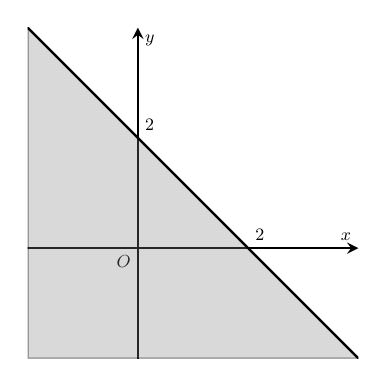
\begin{tikzpicture}[join = round, cap = round, >=stealth, thick,transform shape, font = \small, scale = 0.7]
			\clip (-2,-2) rectangle (4,4);
			\draw[->](-2,0) --(0,0)node[below left]{$O$}-- (4,0)node[above left]{$x$};
			\draw[->](0,-2) -- (0,4)node[below right]{$y$};
			\draw[fill=black!50,opacity=0.3](-2,4)--(-2,-2)--(4,-2)--(-2,4)--cycle;
			\draw(-2,4)--(4,-2);
			\draw(2,0)node[above right]{$2$} 
			(0,2)node[above right]{$2$};
		\end{tikzpicture}
	}
	\loigiai{
		Miền nghiệm không bị gạch chéo, không kể cả bờ, chỉ ra rằng đường thẳng $ x+y=2 $ không thuộc miền nghiệm. \\
		Vì miền nghiệm không chứa $O(0;0)$ nên, bất phương trình tương ứng phải là $ x+y>2 $.
	}
\end{ex}

%[Câu 16]
\begin{ex}% [0H4H2-1][Dự án đề kiểm tra Toán 11 GHKI NH23-24- Dung Mai Dung]%[THPT Nguyễn Du- Tp HCM]
	Cho tam giác $ABC$ có cạnh $BC=5$, góc $\widehat{BAC}=60^{\circ}$ và $\widehat{ACB}=45^{\circ}$. Tính độ dài cạnh $AB$.
	\choice
	{$\dfrac{5 \sqrt{2}}{3}$}
	{$\dfrac{5 \sqrt{3}}{3}$}
	{\True $\dfrac{5 \sqrt{6}}{3}$}
	{$\dfrac{ \sqrt{6}}{3}$} 
	\loigiai{
		Áp dụng định lý sintrong tam giác $ABC$:
		\[\dfrac{AB}{\sin C} = \dfrac{BC}{\sin A}.\]
		Suy ra:
		\[AB = \dfrac{5 \sin 45^{\circ}}{\sin 60^{\circ}} = \dfrac{5\sqrt{6}}{3}.\]
	}
\end{ex}

%[Câu 17]
\begin{ex}%[0D1H1-1][Dự án đề kiểm tra Toán 11 GHKI NH23-24- Dung Mai Dung]%[THPT Nguyễn Du- Tp HCM]
	Trong các câu sau, câu nào là mệnh đề không chứa biến?
	\choice
	{\True $10$ là số chính phương}
	{$a+b=c$}
	{$2n+1$ chia hết cho $3$}
	{$x^2-x=0$}
	\loigiai{
		Một mệnh đề là một câu phát biểu cụ thể có thể xác định rõ ràng là đúng hoặc sai. Trong các lựa chọn:
		\begin{itemize}
			\item Câu "$10$ là số chính phương" là một mệnh đề không chứa biến vì nó không phụ thuộc vào bất kỳ biến số nào và có thể được xác định rõ ràng là sai.
			\item Các câu còn lại đều chứa biến và không thể xác định là đúng hoặc sai mà không cần thêm thông tin về giá trị của các biến.
		\end{itemize}ư
		
	}
\end{ex}

%[Câu 18]
\begin{ex}%[0D1H1-1][Dự án đề kiểm tra Toán 11 GHKI NH23-24- Dung Mai Dung]%[THPT Nguyễn Du- Tp HCM]
	Trong các khẳng định sau, có bao nhiêu khẳng định là mệnh đề?
	\begin{itemize}
		\item $2+4=7$.
		\item Học, học nữa, học mãi.
		\item Hình chữ nhật có hai đường chéo cắt nhau tại trung điểm mỗi đường.
		\item Tam giác có hai đường cao bằng nhau là tam giác cân.
	\end{itemize}
	\choice
	{\True $3$}
	{$4$}
	{$2$}
	{$1$}
	\loigiai{
		Một mệnh đề là một khẳng định có thể xác định được tính đúng hoặc sai của nó.
		\begin{itemize}
			\item $2+4=7$ là một mệnh đề, vì có thể xác định được nó là sai.
			\item "Học, học nữa, học mãi." không phải là một mệnh đề, vì đây là một lời khuyên, không thể xác định được tính đúng hoặc sai.
			\item "Hình chữ nhật có hai đường chéo cắt nhau tại trung điểm mỗi đường." là một mệnh đề và là một mệnh đề đúng, vì nó mô tả một tính chất của hình chữ nhật có thể được kiểm chứng.
			\item "Tam giác có hai đường cao bằng nhau là tam giác cân." cũng là một mệnh đề, và nó là đúng vì nó mô tả một tính chất có thể kiểm chứng của tam giác cân.
		\end{itemize}
		Vậy có 3 khẳng định trong số các khẳng định trên là mệnh đề.
	}
\end{ex}

%[Câu 19]
\begin{ex}%[0D2V1-2][Dự án đề kiểm tra Toán 11 GHKI NH23-24- Dung Mai Dung]%[THPT Nguyễn Du- Tp HCM]
	Miền nghiệm (phần không bị gạch chéo) của bất phương trình $3x-2y>-6$ là
	\choice
	{ \begin{tikzpicture}[scale=1, font=\footnotesize, line join=round, line cap=round, >=stealth]
			\begin{scope}
				\clip (-1,-1) rectangle (4,4);
				\fill[pattern=north east lines] (-2/3,4)--(-1,4)--(-1,-1)--(4,-3)--cycle;
				\draw (-2/3,4)--(4,-3);
			\end{scope}
			\draw[->] (-1,0)--(4.1,0) node[right]{$x$};
			\draw[->] (0,-1)--(0,4.2) node[above]{$y$};
			\draw (0,0) node[below left]{$O$};
			\foreach \x in {2}
			\draw[thin] (\x,1pt)--(\x,-1pt) node [above right] {$\x$};
			\foreach \y in {3}
			\draw[thin] (1pt,\y)--(-1pt,\y) node [above right] {$\y$};
	\end{tikzpicture}}
	{ \begin{tikzpicture}[scale=1, font=\footnotesize, line join=round, line cap=round, >=stealth]
			\begin{scope}
				\clip (-1,-1) rectangle (4,4);
				\fill[pattern=north east lines] (-2/3,4)--(4,4)--(4,0)--(4,-3)--cycle;
				\draw (-2/3,4)--(4,-3);
			\end{scope}
			\draw[->] (-1,0)--(4.1,0) node[right]{$x$};
			\draw[->] (0,-1)--(0,4.2) node[above]{$y$};
			\draw (0,0) node[below left]{$O$};
			\foreach \x in {2}
			\draw[thin] (\x,1pt)--(\x,-1pt) node [below left] {$\x$};
			\foreach \y in {3}
			\draw[thin] (1pt,\y)--(-1pt,\y) node [left] {$\y$};
	\end{tikzpicture}}
	{\True \begin{tikzpicture}[scale=1, font=\footnotesize, line join=round, line cap=round, >=stealth]
			\begin{scope}
				\clip (-3,-4) rectangle (2,4);
				\fill[pattern=north east lines] (2/3,4)--(-8/3,4)--(-8/3,-1)--cycle;
				\draw (2/3,4)--(-8/3,-1);
			\end{scope}
			\draw[->] (-2.7,0)--(1,0) node[above]{$x$};
			\draw[->] (0,-1)--(0,4) node[right]{$y$};
			\draw (0,0) node[below left]{$O$};
			\foreach \x in {-2}
			\draw[thin] (\x,1pt)--(\x,-1pt) node [below right] {$\x$};
			\foreach \y in {3}
			\draw[thin] (1pt,\y)--(-1pt,\y) node [right] {$\y$};
	\end{tikzpicture}}
	{\begin{tikzpicture}[scale=1, font=\footnotesize, line join=round, line cap=round, >=stealth]
			\begin{scope}
				\clip (-3,-4) rectangle (2,4);
				\fill[pattern=north east lines] (2/3,4)--(2/3,-1)--(-8/3,-1)--cycle;
				\draw (2/3,4)--(-8/3,-1);
			\end{scope}
			\draw[->] (-3,0)--(0.8,0) node[above]{$x$};
			\draw[->] (0,-1)--(0,4) node[right]{$y$};
			\draw (0,0) node[below left]{$O$};
			\foreach \x in {-2}
			\draw[thin] (\x,1pt)--(\x,-1pt) node [above left] {$\x$};
			\foreach \y in {3}
			\draw[thin] (1pt,\y)--(-1pt,\y) node [left] {$\y$};
	\end{tikzpicture}}
	
	\loigiai{
		\immini{Đường thẳng $3x-2y=-6$ đi qua hai điểm $( -2;0 ),( 0;3 )$.
			Mặt khác $O( 0;0 )$ thỏa mãn $3x-2y>-6$ nên $O$ thuộc miền nghiệm. Vậy chọn đáp án hình bên.}{\begin{tikzpicture}[scale=1, font=\footnotesize, line join=round, line cap=round, >=stealth]
				\begin{scope}
					\clip (-3,-4) rectangle (2,4);
					\fill[pattern=north east lines] (2/3,4)--(-8/3,4)--(-8/3,-1)--cycle;
					\draw (2/3,4)--(-8/3,-1);
				\end{scope}
				\draw[->] (-2.7,0)--(1,0) node[above]{$x$};
				\draw[->] (0,-1)--(0,4) node[right]{$y$};
				\draw (0,0) node[below left]{$O$};
				\foreach \x in {-2}
				\draw[thin] (\x,1pt)--(\x,-1pt) node [below right] {$\x$};
				\foreach \y in {3}
				\draw[thin] (1pt,\y)--(-1pt,\y) node [right] {$\y$};
			\end{tikzpicture}
		}
		
	}
\end{ex}

%[Câu 20]
\begin{ex}%[0D1H2-1][Dự án đề kiểm tra Toán 11 GHKI NH23-24- Dung Mai Dung]%[THPT Nguyễn Du- Tp HCM]
	Cho tập hợp $A=\{2x+3 \mid x \in \mathbb{N}, x \leq 5\}$. Tập hợp $A$ là
	\choice
	{\True $\{3; 5; 7; 9; 11; 13\}$}
	{$\{1; 3; 5; 7; 9; 11\}$}
	{$\{3; 7; 11; 15; 19; 23\}$} % Giả sử đây là đáp án đúng sau khi tính toán
	{$\{0; 1; 2; 3; 4; 5\}$}
	\loigiai{
		Tập hợp $A$ được xác định bằng các phần tử có dạng $2x+3$ với $x$ là số tự nhiên không lớn hơn $5$. Ta liệt kê các giá trị của $x$ từ $0$ đến $5$:
		\begin{itemize}
			\item Với $x=0$, ta có $2 \cdot 0 + 3 = 3$.
			\item Với $x=1$, ta có $2 \cdot 1 + 3 = 5$.
			\item Với $x=2$, ta có $2 \cdot 2 + 3 = 7$.
			\item Với $x=3$, ta có $2 \cdot 3 + 3 = 9$.
			\item Với $x=4$, ta có $2 \cdot 4 + 3 = 11$.
			\item Với $x=5$, ta có $2 \cdot 5 + 3 = 13$.
		\end{itemize}
		Vậy, đáp án đúng phải là $\{3; 5; 7; 9; 11; 13\}$.
	}
\end{ex}

\Closesolutionfile{ans}
%\begin{center}
%	\textbf{ĐÁP ÁN}
%	\inputansbox{10}{ans/ans}	
%\end{center}


\begin{center}
	\textbf{PHẦN 2 - TỰ LUẬN}
\end{center}

%Câu 1...........................
\begin{bt}%[0D1H2-1]%[Dự án đề kiểm tra Toán 10 GHKI NH23-24- Tư Đô Nguyên]%[THPT Nguyễn Du- Tp HCM]
	Cho tập hợp $A=\left\{x \in \mathbb{Z} \mid \left(2x^2+5x+2\right)\left(x^2-16\right)=0\right\}$. Tìm tập hợp $A$ được viết dưới dạng liệt kê.
	\loigiai{
	Ta có
	\allowdisplaybreaks
	\begin{eqnarray*}	\left(2x^2+5x+2\right)\left(x^2-16\right)=0 \Leftrightarrow \hoac{&2x^2+5x+2=0 \\ &x^2-16=0} \Leftrightarrow \hoac{&x=-\dfrac{1}{2} \not\in \mathbb{Z}\\
	&x=-2 \in \mathbb{Z}\\ &x=\pm 4 \in \mathbb{Z}}
	\end{eqnarray*}
	Do đó, tập hợp $A$ viết dưới dạng liệt kê $A=\left\{-4;2;4\right\}$.
	}
\end{bt}

\begin{bt}%[0H4H2-2]%[Dự án đề kiểm tra Toán 10 GHKI NH23-24- Tư Đô Nguyên]%[THPT Nguyễn Du- Tp HCM]
	\immini{
		Từ công thức diện tích $S=\dfrac{1}{2}a\cdot h_a$ của tam giác $ABC$ (tham khảo hình vẽ bên), hãy chứng minh diện tích tam giác $ABC$ còn được tính theo công thức $S=\dfrac{1}{2}ab\sin C$.%Điền câu hỏi
	}
	{
\begin{tikzpicture}[scale=1,nodes={scale=1}]
	\path (0,0) coordinate (B) 
	(4,0) coordinate (C) (1,2) coordinate (A) 
	($(B)!(A)!(C)$) coordinate (H);
	\draw (A)--(B)node[pos=.5,above left]{$c$};
	\draw (B)--(C)node[pos=.7,below]{$a$};
	\draw (C)--(A)node[pos=.5,above]{$b$};
	\draw (A)--(H)node[pos=.5,right]{$h_a$};
	\draw pic[draw,angle radius=3mm]{right angle=C--H--A};
	\foreach \x/\g in {A/90,B/180,C/-45,H/-90}
			\fill[black] 	(\x) circle (1pt)
			($(\g:3mm)+(\x)$) node {$\x$};
	\draw pic[draw,,angle radius=5mm]{angle=A--C--B};%Theo chiều dương, tùy chọn double,fill=yellow!50,-stealth,dashed

	
\end{tikzpicture}
	}
		\loigiai{
		Xét $\triangle AHC$ vuông tại $H$ ta có $\sin C=\dfrac{AH}{AC}=\dfrac{h_a}{b} \Leftrightarrow h_a=b\sin C$. \\
		Khi đó $S=\dfrac{1}{2}a\cdot h_a=\dfrac{1}{2}a \cdot \left(b \sin C\right)=\dfrac{1}{2}ab\sin C$.
	}
\end{bt}
\begin{bt}%[0H4V2-1]%[Dự án đề kiểm tra Toán 10 GHKI NH23-24- Tư Đô Nguyên]%[THPT Nguyễn Du- Tp HCM]
	Cho hình vuông $ABCD$ có độ dài cạnh bằng $8$, $M$ là trung điểm của $CD$. Tìm bán kính đường ngoại tiếp tam giác $ACM$.
	\loigiai{
	\begin{center}
		\begin{tikzpicture}
	\def\a{3} %cạnh
	\path (0:0) coordinate (B)
			++(0:\a) coordinate (C)
			++(90:\a) coordinate (D)
			++(180:\a) coordinate (A)
			($(C)!.5!(D)$) coordinate (M)
			;
	\draw (A)--(B)--(C)--(D)--cycle (M)--(A)--(C) ;
	\foreach \x/ \goc in {A/135,B/-135,C/-45,D/45,M/0} 
			\fill (\x) circle (1pt)
			($(\x)+(\goc:3mm)$) node {$\x$};
	\end{tikzpicture}
	\end{center}
	Ta có độ dài cạnh $AM=\sqrt{AD^2+DM^2}=\sqrt{8^2+4^2}=4\sqrt{5}$. \\
	Áp dụng định lí sin cho $\triangle ACM$ ta có: $$\dfrac{AM}{\sin\widehat{ACM}}=2R \Leftrightarrow R=\dfrac{AM}{2\sin\widehat{ACM}}=\dfrac{4\sqrt{5}}{2\sin 45^\circ}=2\sqrt{10}.$$
	}
\end{bt}

\begin{bt}%[0H4V3-2]%[Dự án đề kiểm tra Toán 10 GHKI NH23-24- Tư Đô Nguyên]%[THPT Nguyễn Du- Tp HCM]
	\immini{
	Hai máy bay cùng cất cánh từ một sân bay nhưng bay theo hai hướng khác nhau. Một chiếc di chuyển với tốc độ $500$ km/h theo hướng tây và chiếc còn lại di chuyển theo hướng lệch so với hướng bắc $35^\circ$ về phía tây với tốc độ $650$ km/h. Sau 90 phút, hai máy bay cách nhau bao nhiêu kilômét? Giả sử chúng đang ở cùng độ cao.	%Điền câu hỏi
	}
	{
	\begin{tikzpicture}[scale=0.7, font=\footnotesize, line join=round, line cap=round, >=stealth]
		\path
		(0,0) coordinate (A)
		(6,0) coordinate (O)
		(3,5) coordinate (B)
		;
		\draw (A) -- (O) -- (B);
		\draw [dashed] (A) -- (B);
		\fill[black](O) circle (1.5pt);
		\draw (B) node [above]{B}
		(O) node [right]{O}
		(A) node [below]{A};
		\draw (A) -- (O) node [sloped,midway,below]{$500$ km/h}; 	
		\draw (B) -- (O) node [sloped,midway,below]{$650$ km/h};
		\draw [->] (O)--(A);
		\draw [->] (O)--(B);
		\draw [->] (O)--(6,5);
		\draw (-0.5,0) node{Tây} (6,5) node[above]{Bắc};
		\draw (5.6,1.5) node{$35^\circ$};
	\end{tikzpicture}	%Chèn hình
	}
	\loigiai{
	Sau $90$ phút:
	\begin{itemize}
		\item Máy bay đầu tiên bay được $\dfrac{500\cdot 90}{60}= 750$ km.
		\item Máy bay thứ hai bay được $\dfrac{650\cdot 90}{60}= 975$ km.
	\end{itemize}
	Hai máy bay di chuyển lệch nhau một góc $90^\circ - 35^\circ = 55^\circ$.\\
	Ta có tam giác $ABO$ với $OA=750$ km, $OB=975$ km và $\widehat{BOA}=55^\circ$.\\
	Áp dụng định lí côsin, ta có
	\[AB^2=OA^2+OB^2-2\cdot OA \cdot OB \cdot \cos \widehat{BOA}=750^2+975^2-2\cdot 750 \cdot 975 \cdot \cos 55^\circ \approx 674\;269{,}46.\]
	Suy ra $AB=\sqrt{674\;269{,}46}\approx 821{,}14$ km.\\
	Vậy sau $90$ phút hai máy bay cách nhau	$821{,}14$ km.
	}
	
\end{bt}